\documentclass[12pt]{article}

\usepackage{graphicx}	
\usepackage{hyperref}

%%%%%%%%%%%%%%%%%%%%%%%%%%%%%%%%%%

\title{Web Design Documentation}											
\author{Shalini Denti,}
\date{08.11.2026}

%%%%%%%%%%%%%%%%%%%%%%%%%%%%%%%%%%
\begin{document}



\section{Introduction:}
	
	Whether you are a digital designer, a business leader or a product manager, there’s one thing is important in the process: 
	make the product the most accessible for a larger set of costumers. This includes also the way you interact through the interface
	 of a computer to display information as simple as possible for the costumer, in order to get its attention and let him focus on the
	  valuable information. Not all human are equal in some capacity regarding the sense or the way their mind work. This is the 
	  reason it is needed to accomplish design elements to let the largest amount of people understand what does the screen display 
	  and how to easily interact with it.

	In this section we’re going to first do an overview, to understand where this necessities came from, and then the various 
	subtopics.
	
	\begin{enumerate}
		\item Historical part
		\item Divers users needs
	\end{enumerate}

	\begin{figure}[h]										
	\centering
			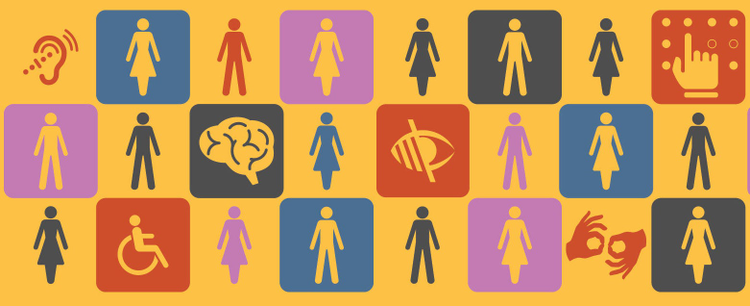
\includegraphics [width=10cm]{Accessibility_design_introduction.png}	
			\caption{fig.2.1}
	\end{figure}
	
\subsection{Defining inclusive design in the digital era:}

	As technologies is becoming more and more central in daily life, and the expansion of tech market is enlarging even more, 
	there’s the need to provide to everyone a simple approach of any digital technologies in a digital society.
	It all started back then, when computers were slow machines with low comprehension of inputs of the user and very complex 
	interface. In a nutshell, The computer accessibility was quite complicated and difficult to understand. As the spectrum of human 
	diversity and capacities deepen, also the design approach evolve too. With the birth of World Wild Web the challenge was set:  
	many web pages had changed styles and tools to be more understandable and approachable for users.  Features like keyboard 
	navigation, alternative text for images and other tools that are now the default set of a web page. by the end of 90’s there was an
	 historical improvement with the publication of “Web Accessibility guidelines” where a crucial standard was set and developers 
	 could use a shared framework . All for one goal: make web sites easier. 

	Another key accomplishment is approved when web designer shifted from “designing for disabilities” to “design for diversity”.
	Before, designers were designing special features with the only purpose to help disabled people to use interface and other 
	technologies. Even though it was the first and crucial step to help these people, these disability-specific adaptations were 
	targeting
	 disabled people as different. A few times later, designers realized that a bunch of more people could get benefits from some 
	 disability-specific adaptations and conclude that the variants they created could be extended to a more large set of people.
	
	For example: Voice control features designed in principle for people with motor disabilities, nowadays they become convenient 
	 for multitasking parents with their hands full or drivers needing an hand - free operation. So diversity instead of disability.
	 
	 \begin{figure}[h]										
	\centering{
		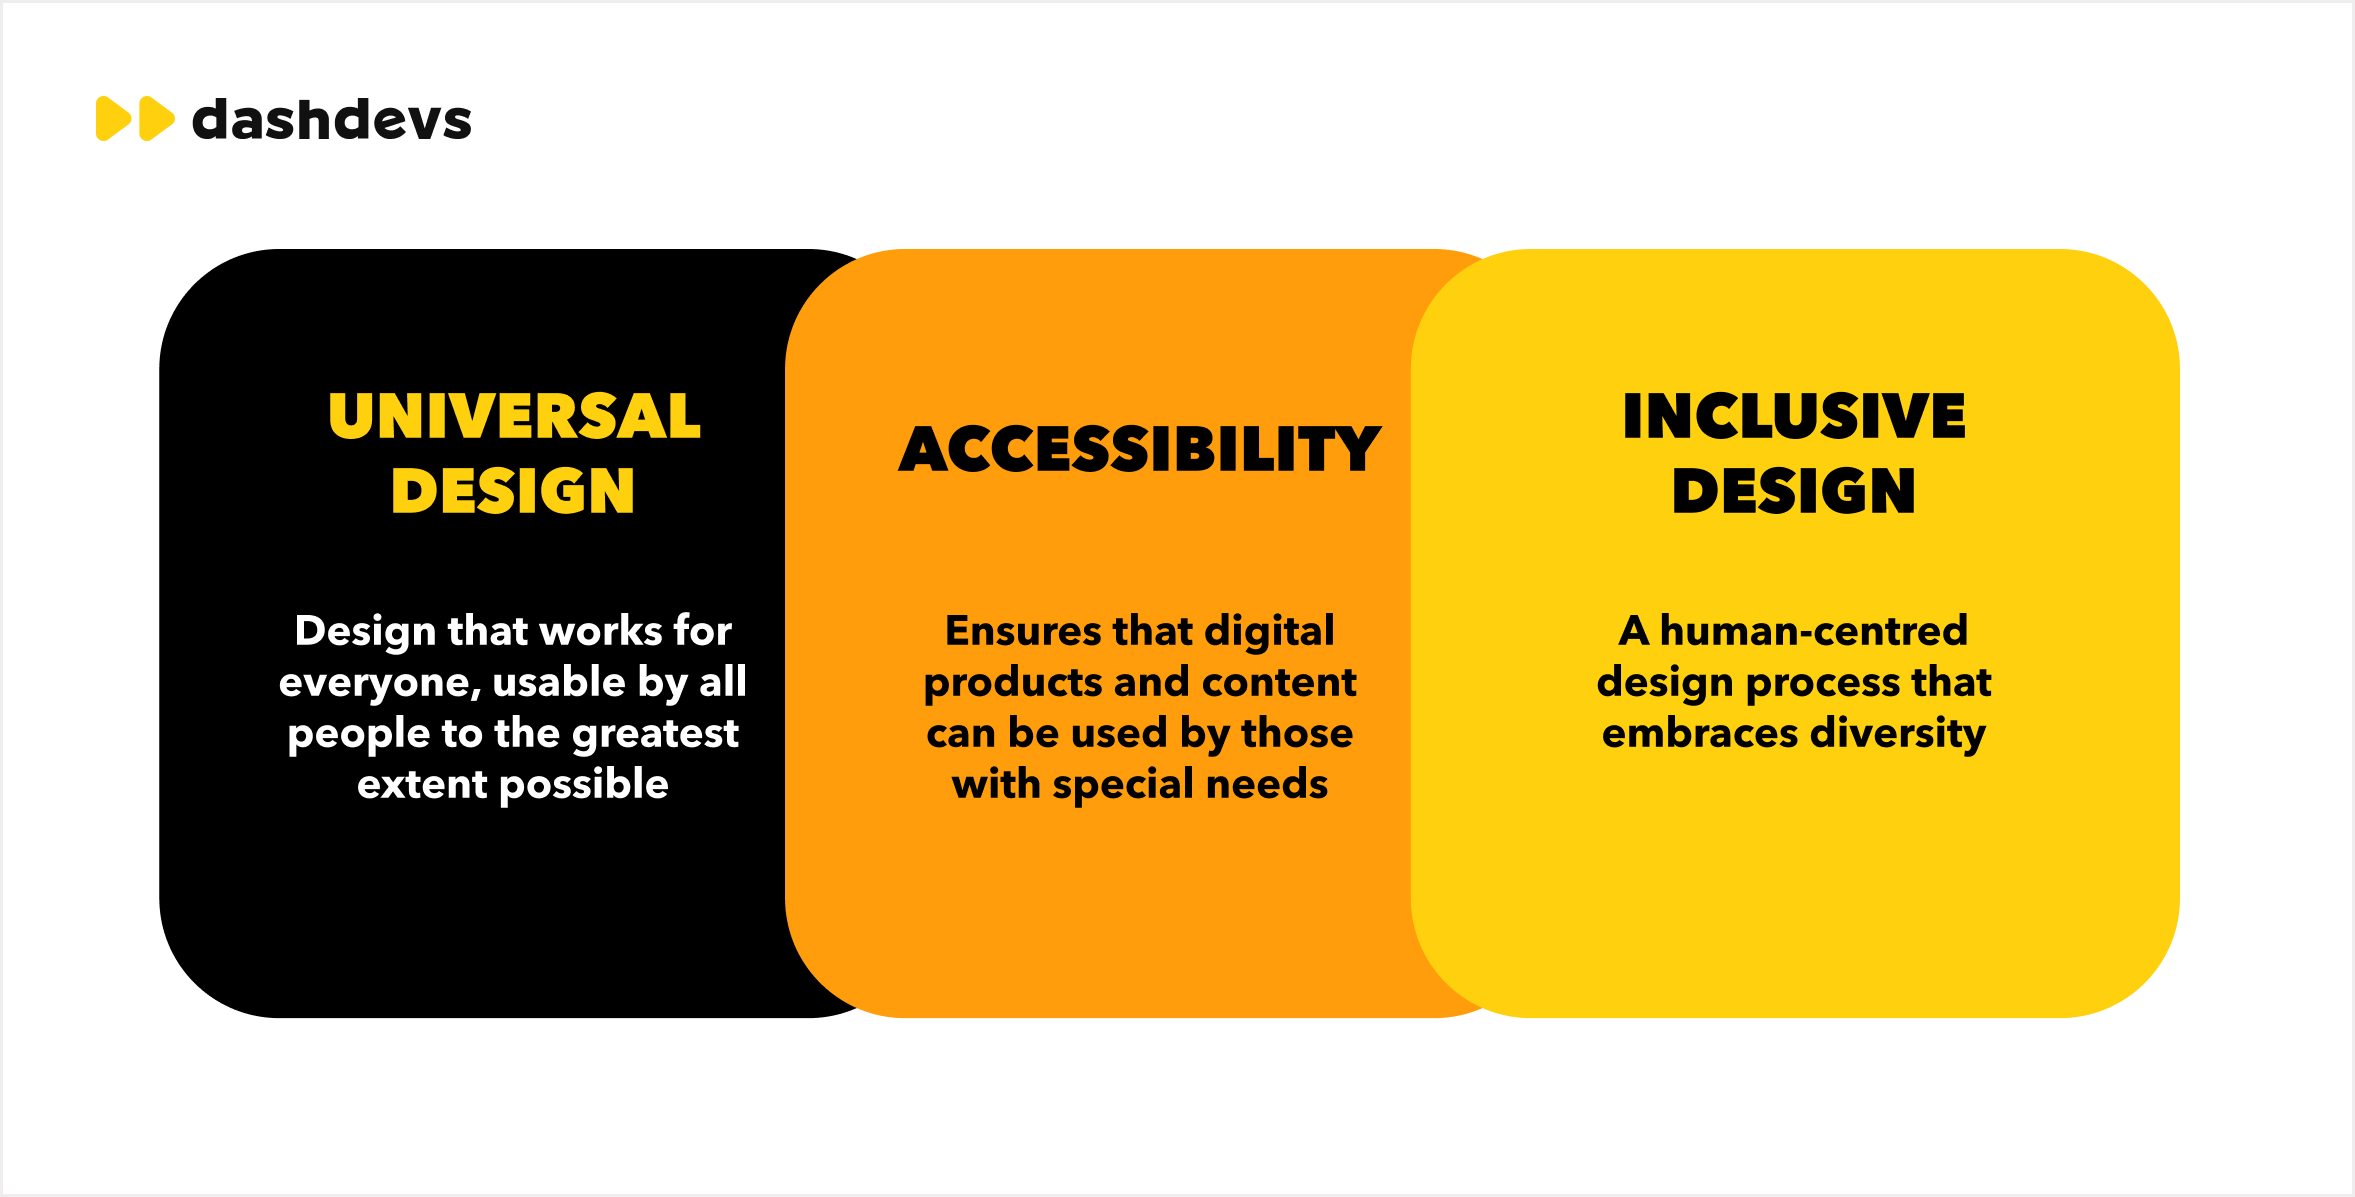
\includegraphics [width=10cm]{value-adding-benefits-of-mobile-friendly-website-design.jpg}
		\caption{fig.2.2}
	}	
	\end{figure}
	 
	 It is also fair to say that nowadays everyone can have a disability based on the personal condition or the environment they’re in: 
	  a commuter in a bumpy bus, a broken arm, or else; which differs from the historical definition which marked a person as 
	  fundamentally different from a normal one. Now for any reasons a person cannot do their task properly. This is why everyone 
	  can 
	  benefits from the upgrade of digital system performances: to make everyday challenges smoother for everyone.

	In the modern world the disability is not something you are born with until you are in an environment not thought for your needs 
	or your personal shortcomings. This change of mind include a different approach in the code script: it’s not anymore the individual 
	in charge to conform to others but quite the opposite, it’s the society who must conform to itself; hence the web must change for
	 users and users are not required to change or acknowledge things to understand the web. We can say that now is more of full 
	 set 
	 of people oriented and not only for those few smart people. We can create now a digital space that welcome everyone, 
	 regardless 
	 the ability.
	 	  
		 

\subsection{Divers user needs:}

	Types of disabilities and Assistive technologies

	The key of this challenge is first to understand and recognize the divers spectrum of user needs and abilities. In order to 
	acknowledge this concept, the book is marking some clue concept we can summarize in here:
	
	\begin{enumerate}
		\item  Types of disabilities: recognize the duration of disability: temporally, permanent or due to the situation.
		\item Accessibility spectrum: since the accessibilities can be very different and various, the design need to be really 
		flexible to provide solutions for different kind of ability levels. For example adjustable font-size of words.
		\item Intersectionality: Considering the existence of multiple factors can compound accessibility challenges. 
		If some users has more than one shortcomings.
		\item Changing needs: User needs can evolve during time, this put an highlight on elder people who may be limited 
		in mobility and need the web to accommodate their needs.
		\item Cultural diversity: User cultural and linguistic differences can also make improvements in accommodating needs 
		and enlarge the additional tools for people-disabilities orientation. 
	\end{enumerate}

	Seven principles of universal design:
	It is required a deep knowledge of how different people navigate the digital world.
	Another fundamental concepts are the seven principles of universal design:
	
	\begin{enumerate}
		 \item Equitable use: A website must let everyone decides whether they want to adjust the text size and color contrast 
		 based on their preference.
		 \item Flexibility in use: The web sites let you decide you kind of interaction with interface: whether you tap, type or talk. 
		 It is better if it include either fingertips or voice commands.
		\item Simple and inductive use: Simplicity and effectiveness over anything else.
		 \item Perceptible information: A video player offering captions, audio description or else, that ensure you won’t misses 
		 any information.
		\item Tolerance for error: nicely provide to show you your errors without making you feel dumb.
		\end{enumerate}
		
	Low physical effort: implementing shortcuts and content management with bulk actions in order to make every task simpler
	
	 
	 \begin{figure}[h]										
	\centering{
		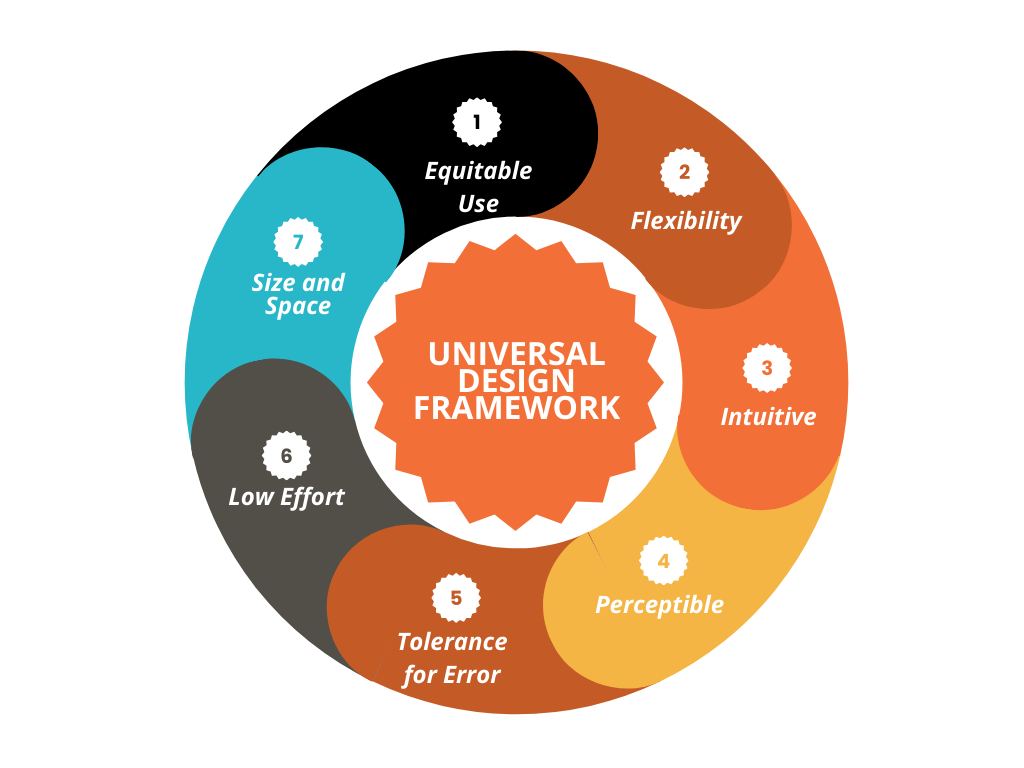
\includegraphics [width=10cm]{Universal-Design-Framework.png}
		\caption{2.3}
	}	
	\end{figure}
	
	By prioritizing inclusivity from the star, we create digital environments that not only meet diverse needs but also foster innovation
	 and connection of everyone. Let’s group them into categories:
	 
	 \begin{enumerate}
 		\item Visual disabilities: for user who are blind or has a restricted vision it’s essential that an audio form or a more larger size 
		can be fundamentals. Playing also with highlighted words can be really useful and an ordered paragraph can be the key of a 
		better comprehension instead of a chaotic unique paragraph text with no labeling and no images. Alternative method are 
		implementing to solve this problem as zoom for screen.
		 \item Auditory disabilities: Such as deaf or compromised hearing. It is required alternatives for video or anything that 
		 includes sounds such as transcription of the video. In this case are also used flashing-lights as Set Alarm to ensure that the 
		 information can reach beyond the hearing ability.
		 \item Motor disabilities: can include such as tremor or arthritis to paralysis and amputation. These conditions can affect how
		  people interact with digital device. A solution can be voice interaction, but for those who also have that kind of disabilities it 
		  must be implemented other kind of inputs.
		  \item  Cognitive disabilities: for example dyslexia or ADHD, compromise user perception and information can’t be 
		  absorbed. Of course there are many solutions like a more interactive web sites with many intuitive figures that provide 
		  visual clarity without overstimulating the user.
	\end{enumerate}

%%%%%%%%%%%%%%%%%%%%%%%%%%%%%%%%% Documentation

\section{links}
	
	\begin{itemize}
	\item Subtopic 2:  \url{https://books.google.ch/books?hl=it&lr=&id=qaNxEQAAQBAJ&oi=fnd&pg=PP1&dq=Interface,+inclusive+design+principles&ots=N3sSFD2wu6&sig=joiCB_Rtm_UsUrDiABZb9EwNItE&redir_esc=y#v=onepage&q&f=true}
	\end{itemize}

\section{images}

	\begin{itemize}
	\item fig.2.1 :  \url {https://blog.adobe.com/en/publish/2018/04/02/different-breaking-accessibility-universality-inclusion-design}
	\item fig.2.2 :  \url{https://dashdevs.com/blog/inclusive-design-and-ux-accessibility/}
	\item fig.2.3 :  \url{https://www.singlegrain.com/blog-posts/design/design-principles-for-accessibility/}
	\end{itemize}



\end{document}
